\pgfplotsset{
    colormap={whitered}{
        color(0cm)=(white);
        color(1cm)=(orange!75!red)
    }
}
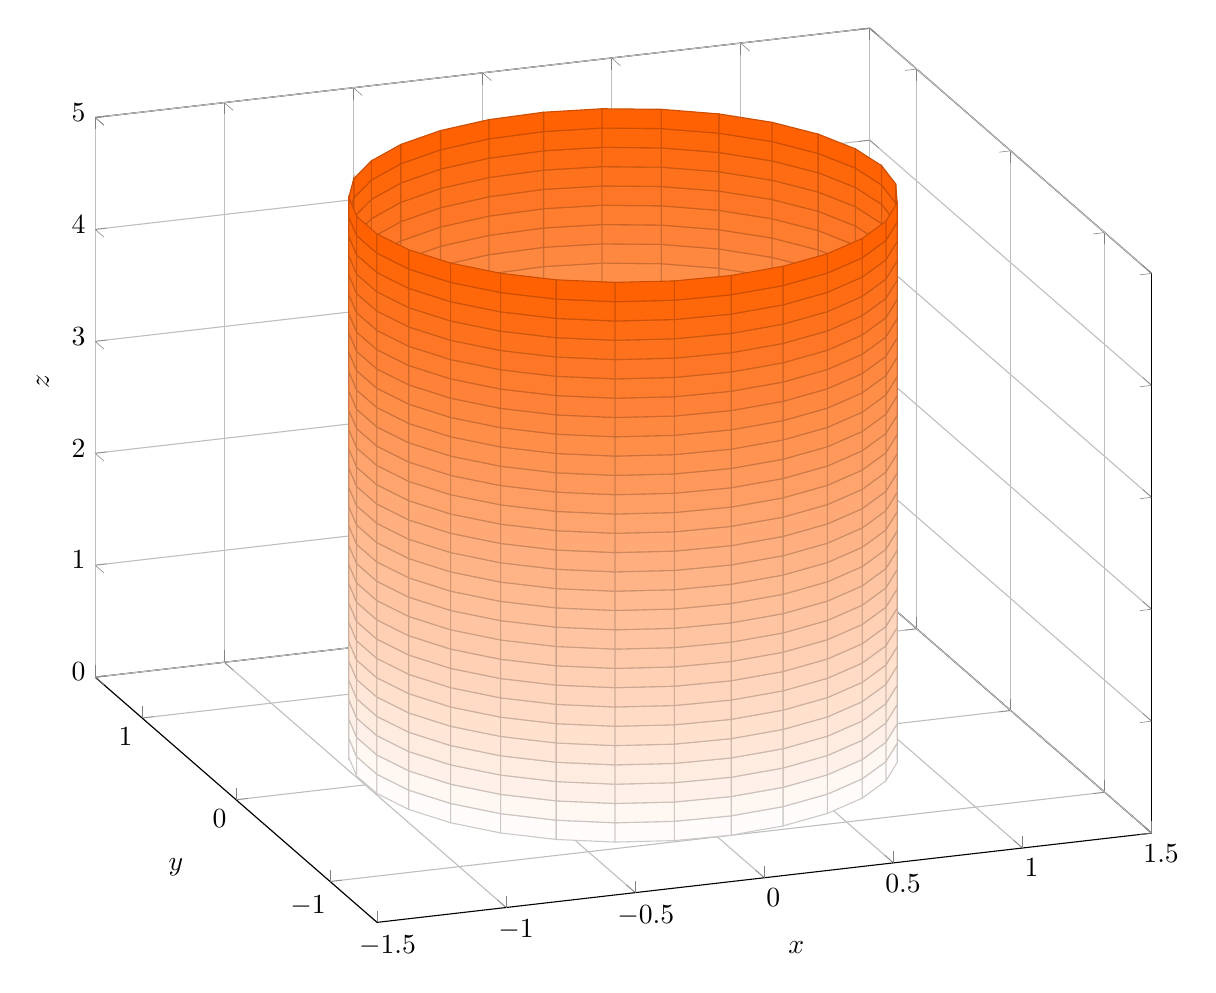
\begin{tikzpicture}
    \begin{axis}[
    colormap name=whitered,
    width=15cm,
    view={340}{25},
    enlargelimits=false,
    grid=major,
    domain=0:5,
    y domain=0:2*pi,
    xmin=-1.5, xmax=1.5,
    ymin=-1.5, ymax=1.5,  zmin=0.0,
    samples=30, %57 : TeX capacity exceeded, sorry [main memory size=3000000].
                % see also http://tex.stackexchange.com/a/7954/5645
    xlabel=$x$,
    ylabel=$y$,
    zlabel={$z$},
    %colorbar,
    colorbar style={
        at={(-0.1,0)},
        anchor=south west,
        height=0.25*\pgfkeysvalueof{/pgfplots/parent axis height},
        title={$f(x,y)$}
    }
    ]
    \addplot3 [surf,z buffer=sort] ({cos(deg(y))},{sin(deg(y))},{x});
    \end{axis}
\end{tikzpicture}
